
    
    \chapter{Experiment}
    \label{experiment}
    V~kapitole \ref{navrh} byl specifikován cíl práce a~návrh jak postupovat při řešení. V~této kapitole je popsán navržený experiment a~jeho průběh. Potřebné součásti experimentu jsou účastníci, vhodné pracovní prostředí, podněty, technické vybavení a~software ke zpracování získaných dat.
    
    \section{Cíl experimentu}
    \label{cil_experimentu}
    Experiment byl prováděn za účelem získání datové sady fyziologických dat měřených pomocí nositelné elektroniky. Datová sada by měla obsahovat průběhy signálů pro zvolené emoce. Předpoklady o~získaných datech před začátkem experimentu:
    \begin{enumerate}
        \item Počet vzorků pro každou emoci bude přibližně stejný.
        \item Rozložení dat bude ovlivněno pohlavím účastníků.
        \item Pro každou emoci bude napříč získanými vzorky podobnost.
        \item Průběhy signálů budou odlišné v~závislosti na pocítěné emoci.
        \item Správnost dat bude nejméně 80\%.
    \end{enumerate}
    
    Zda byly předpoklady správné, je ověřeno v~kapitole~\ref{vysledky}. 
    
    \section{Pilotní testování}
    V~první fázi experimentu bylo provedeno několik pilotních testů pro ověření funkčnosti implementovaného softwaru, správnosti prezentací obsahující podněty apod. Tyto testy byly rozděleny do dvou skupin:
    \begin{itemize}
        \item Verifikace, validace technických částí experimentu.
        \item Ověření správnosti průběhu experimentu.
    \end{itemize} 
    
    Z~důvodu omezené testovací skupiny jsem první testy prováděl sám. Druhá skupina testů byla prováděna dvěma lidmi. Získaná data během pilotního testování nejsou zahrnuta do datové sady. Účastníci pilotních testů nebyli dále účastníci experimentu.
    
    \subsection{Vyhodnocení pilotních testů}
    První skupina testů odhalila několik chyb, které byly následně opraveny. Zásadní chyba, která byla testy odhalena se týkala volby emoce testovanou osobou a~následné pojmenování souboru dat. Jednalo se o~problém špatné indexace, která způsobila přiřazení špatné emoce k~datovým záznamům. V případě neodhalení chyby by nebylo možné považovat získaná data za validní.
    
    Druha skupina testů napomohla k~úpravě výsledné podoby jednotlivých sezení. Podle zpětné vazby obou členů testovací skupiny došlo k úpravě, či výměně několika stimulů. Jednalo se zejména o~audio podněty, kde bylo nutné upravit úroveň hlasitosti, či nahradit podnět za jiný. Dále se ukázalo, že pro stisk tlačítka je nutné vymezit delší časový úsek. Interval byl prodloužen o~1~sekundu.
    
    
    \section{Zvolené podněty}
    Důležitým prvkem jsou podněty, které budou účastníci experimentu pozorovat a~na které budou reagovat. Jak bylo popsáno v~sekci~\ref{podnety_volba}, uspořádání podnětů se drží schématu s~využitím všech tří navržených úprav (viz obr.~\ref{fig:podnety_ruzna_intenzita}). Podněty jsou rozděleny do 6~prezentací, na základě klasifikace a~podobnosti. Každá prezentace je rozdělena na 6~etap, z~toho 3~etapy tvoří podněty a~zbylé jsou neutrální obrazy pro utlumení emocí a~zklidnění testovaného (viz schéma~\ref{fig:schema_prezentace}). Ačkoliv mohou neutrální obrazy být různé (obrazy krajiny), zvolena byla pouze černá plocha. Obrázky jsou čerpány z~veřejných datasetů GAPED~\cite{gaped} a~OASIS~\cite{oasis}. Dalším typem podnětů jsou videonahrávky a~krátké zvukové stopy. Tyto data, včetně dalších obrázků, byla stažena z~veřejných zdrojů (Pexels\footnote{\url{https://www.pexels.com}}, SoundBible\footnote{\url{https://soundbible.com}}, Zapsplat\footnote{\url{https://www.zapsplat.com}}) pod licencí \emph{Creative Commons}\footnote{\url{https://creativecommons.org/licenses/by/3.0/cz/}}. Celkem bylo využito 13 obrázků, 9~zvuků a~5~videonahrávek. Čas promítání podnětů se pohybuje v~rozmezí~8\,--\,10\,s. Tento časový interval byl zvolen na základě předešlých studií (\ref{emotion_to_physio}), kde jsou použity kratší (6~sekund) i~delší (>25~sekund) časové intervaly a~zvolený interval je tedy v~rozmezí obvyklých hodnot.
    
    \begin{figure}[H]
        \centering
        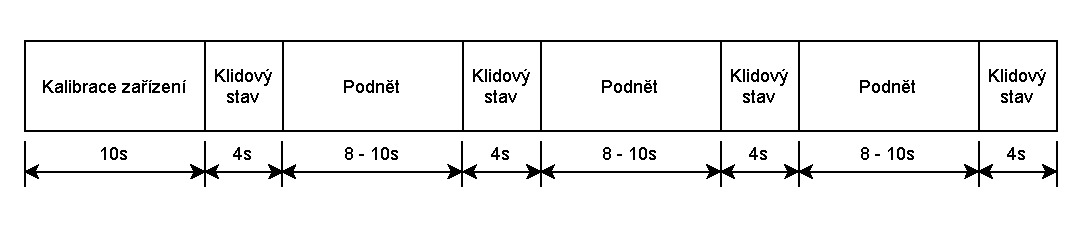
\includegraphics[width=\textwidth]{obrazky-figures/prezentace_schema.pdf}
        \caption{Výsledné schéma prezentací pro experiment. První etapa \uv{Kalibrace zařízení} slouží pro aktivaci senzorů i~uklidnění dobrovolníka před samotným experimentem. Stisk tlačítka je vyžadován před začátkem i~po skončení každé etapy \uv{Klidový stav} vyjma konce poslední této etapy.}
        \label{fig:schema_prezentace}
    \end{figure}
    
    Podstatným problémem použitého schématu je označení časových úseků, kdy má dobrovolník pociťovat emoci a~kdy naopak by měl být v~klidovém stavu. Toho je dosaženo pomocí tlačítka na zařízení E4, které stiskem vysílá signál s~časovou značkou na server. Aby dobrovolník věděl, v~jakém okamžiku stisknout tlačítko, obsahují prezentace slidy s~textem: \uv{Stiskni tlačítko}. Tento způsob řešení však vnáší do dat artefakt, jenž vzniká pohybem zařízení při stisku tlačítka. Jedná se o~krátký impulz na začátku každé etapy, který je nutné filtrovat. Aby nebyla ovlivněna měřená data, je pro stisk vyhrazen delší časový úsek (2~sekundy) a~až poté je promítán další podnět. Délka časového úseku byla stanovena na základě pilotních testů, kde byla uznána jako optimální.
    
    \vspace{3mm}
    
    Neboť nelze předvídat jakou emoci dobrovolník pocítí, probíhá přidělení emoce k~datům až po skončení každé prezentace. Vybrat může ze 6~emocí: 
    \begin{itemize}
        \item nuda,
        \item pozitivní,
        \item radost,
        \item strach,
        \item zmatení,
        \item znechucení.
    \end{itemize}
    
    Jak zobrazuje graf~\ref{fig:emoce_graf} (kapitola~\ref{reserse}), lze emoce rozdělit do 4~kvadrantů. Těchto 6~emocí bylo vybráno tak, aby pokryly všechny 4~kvadranty. 
    
    \begin{table}[H]
    \centering
    \begin{tabular}{|c|c|c|c|c|c|c|}
    \hline
    \begin{tabular}[c]{@{}c@{}}pozitivní, \\
    příjemné
    \end{tabular} & 
    \begin{tabular}[c]{@{}c@{}}radost, \\ 
    smích\end{tabular} & strach & znechucení & zmatek     & \begin{tabular}[c]{@{}c@{}}nuda,\\
    smutek\end{tabular} & klidový stav \\
    \hline  I.                                                             & 
    I.                                                       &
    II.    &
    II.        &
    II. - III. &
    III.                                                   &
    IV.          \\
    \hline
    \end{tabular}
    \caption{Tabulka vybraných emocí přidělených k~jednotlivým kvadrantům podle míry vzrušení a~pozitivity emoce. Součástí tabulky je i~klidový stav.}
    \label{tab:emotion_kvadrants}
    \end{table}
    
    
    \section{Účastníci experimentu}
    Testovací skupina byla složena z~16~členů ($\mu=25$ let, $\sigma=7.6$). Z~toho 9~mužů a~7~žen. Žádný z~účastníků nebyl pod vlivem omamných látek, či léků. Další podmínkou účasti byl zákaz příjmu kofeinu méně než 6~hodin před začátkem sezení. Důvodem je vliv těchto látek na lidský organismus a~ovlivnění fyziologických funkcí. 
    
    
    \section{Pracovní prostředí}
    Pro provedení experimentu byl použit vlastní notebook a~zařízení Empatica E4. Přestože bylo zajištěno klidné prostředí, tak probíhalo přehrávání zvuků pomocí sluchátek za účelem lepší koncentrace. Dále bylo zapotřebí mít software umožňující přehrávání prezentací. Byl zvolen MS PowerPoint\footnote{\url{https://www.microsoft.com/cs-cz/microsoft-365/powerpoint}}. Aby bylo zajištěno větší pohodlí a~uvolněnost účastníků, tak měření probíhala v~domácím prostředí. Tento přístup byl zvolen, neboť všichni účastníci žádný podobný experiment nikdy nepodstoupili a~laboratorní prostředí by mohlo vzbuzovat nervozitu. V~místnosti pro testování se nacházel vždy právě jeden účastník a~dohlížející, který dohlížel na správný průběh měření. Schéma pracovního prostředí zobrazuje obr.\,\ref{fig:pracovni_prostredi}.
    
    \begin{figure}[H]
        \centering
        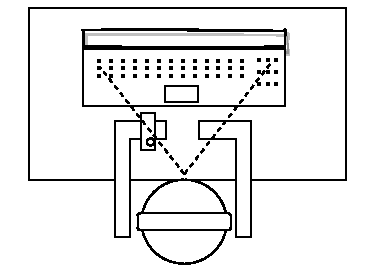
\includegraphics[scale=1.8]{obrazky-figures/pracovni_prostredi.pdf}
        \caption{Schéma pracovního prostředí během experimentu. Aby bylo co nejvíce zamezeno pohybu účastníka, musí mít ruce po celou dobu sezení na stole, co nejblíže u~sebe. To mu umožňuje stisk tlačítka s~minimální fyzickou aktivitou. Náramek je vždy nasazen na levé ruce, neboť na této ruce docházi k~nejmenšímu zpoždění vzhledem k~vzdálenosti od srdce.}
        \label{fig:pracovni_prostredi}
    \end{figure}
    
    \section{Průběh sezení}
    Experiment probíhal jednotlivě v~sezeních, jejichž diagram je zobrazen na obr.\,\ref{fig:session_diagram}. Před začátkem měření proběhl krátký informační rozhovor a~zodpovězení dotazů účastníka. Následně proběhlo samotné měření. Délka jednoho sezení byla přibližně 15 minut. Sezení probíhala v~denní době, kdy byl konkrétní účastník v~čilém stavu, aby data odpovídala běžnému psychickému stavu člověka. 
    
    \begin{figure}[H]
        \centering
        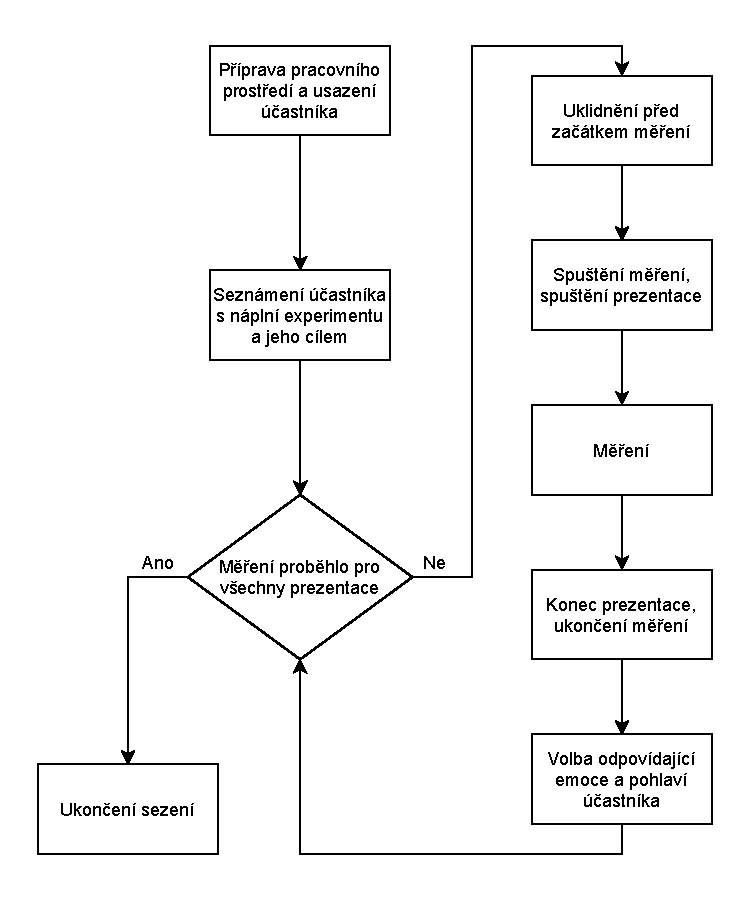
\includegraphics{obrazky-figures/session.pdf}
        \caption{Vývojový diagram průběhu sezení s~účastníkem experimentu.}
        \label{fig:session_diagram}
    \end{figure}
    
    \section{Sběr a~analýza dat}
    Získávání dat a~jejich analýza vyžaduje vlastní software, pro jehož implementaci byl zvolen jazyk Python 3.7\footnote{\url{https://www.python.org}} s~využitím knihoven Pandas\footnote{\url{https://pandas.pydata.org}} a~NeuroKit2~\cite{Makowski2021neurokit}. Naměřená data jsou před zpracováním uložena v~textovém souboru, pojmenována podle schématu složeného ze tří komponent: <EMOCE> <ČA\-SO\-VÁ ZNAČKA VYTVOŘENÍ SOUBORU> <POHLAVÍ>, oddělených podtržítky, kde <EMOCE> i~<POHLAVÍ> jsou volbou účastníka. Od každého testovaného bylo získáno 6~záznamů. Každý záznam obsahuje 3~vzorky fyziologických dat zvolené emoce. Pozorované metriky jsou srdeční tep (PPG signál) a~galvanická odezva kůže (EDA signál). Schéma zpracování zobrazuje obr.\,\ref{fig:data_processing}. Další signály vysílané zařízením jsou zaznamenány, ale nejsou využity. Získaná data jsou blíže popsána v~kapitole~\ref{vysledky}.
    
    \begin{figure}[H]
        \centering
        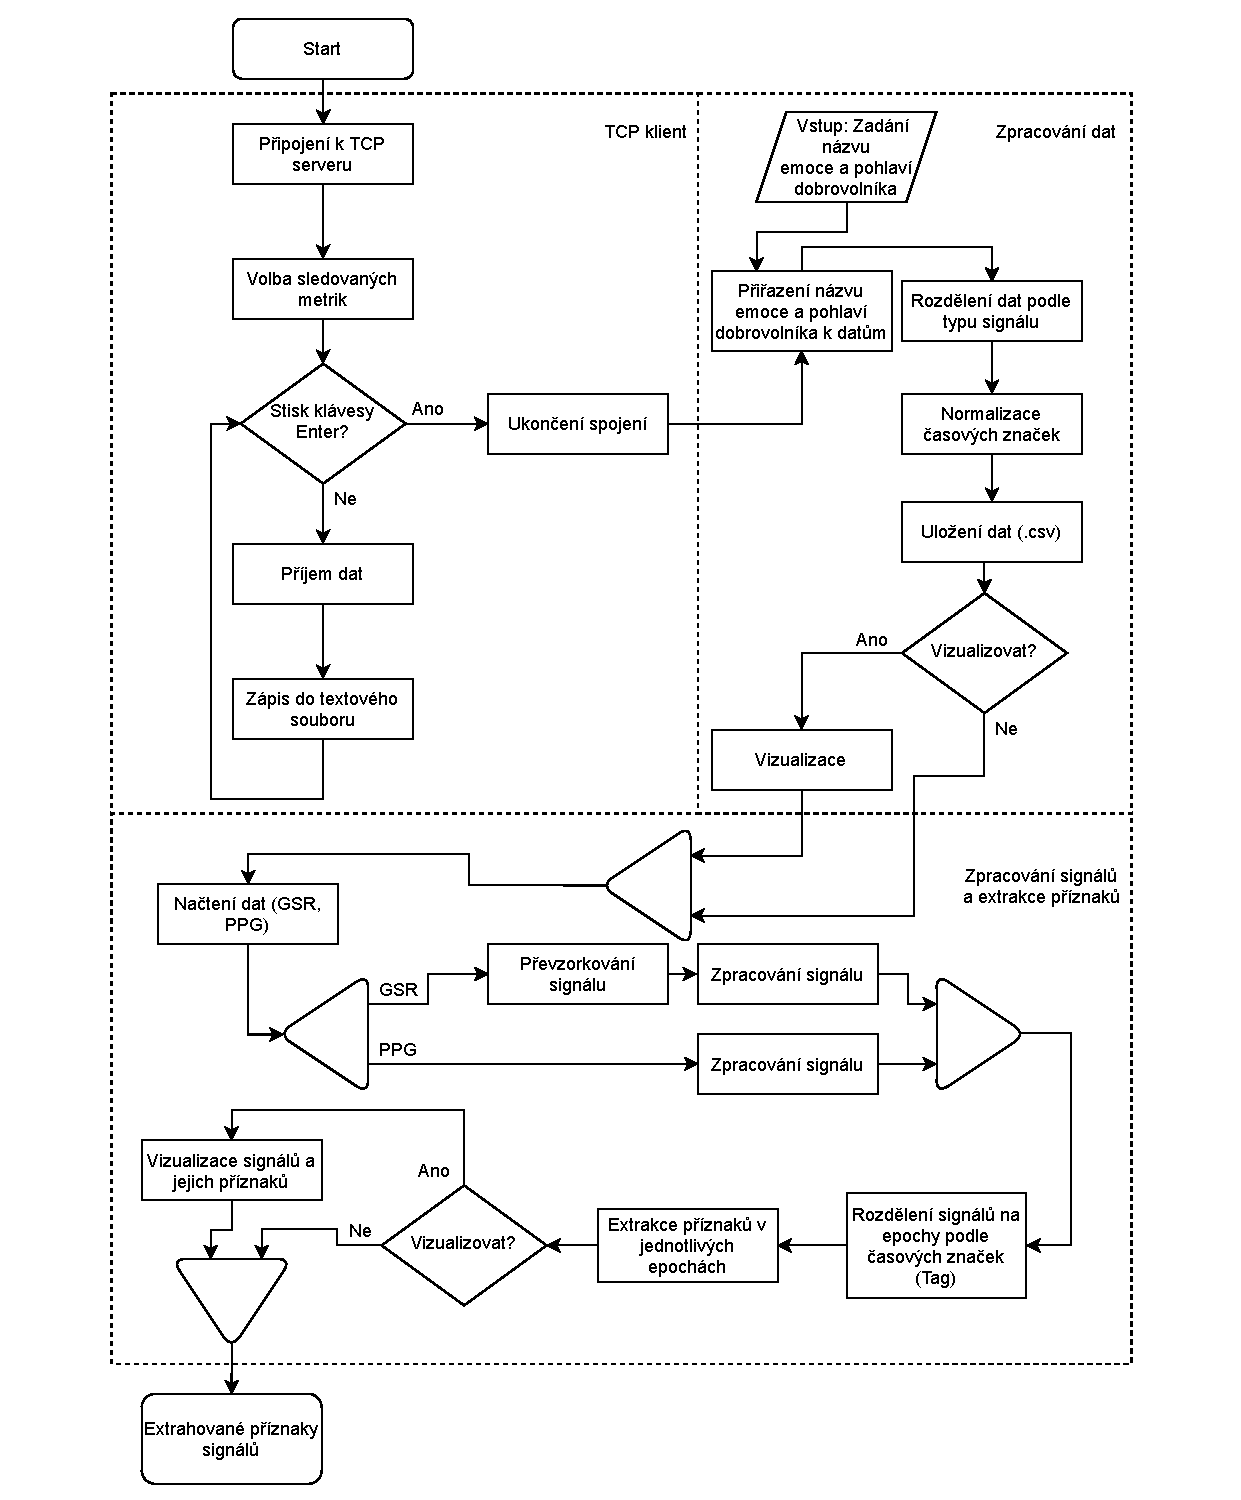
\includegraphics[width=\textwidth]{obrazky-figures/data_processing.pdf}
        \caption{Vývojový diagram zpracování signálů ze zařízení Empatica E4 a~extrakce příznaků ze signálů.}
        \label{fig:data_processing}
    \end{figure}
    
    
    
    
    

    
    
    
    
    
    
    
    
    
    
    
    
    
    
    
    
    
    
    
    
    
    